%%%%%%%%%%%%%%%%%%%%%%%%%%%%%%%%%%%%%%%%%
% Simple Sectioned Essay Template
% LaTeX Template
%
% This template has been downloaded from:
% http://www.latextemplates.com
%
% Note:
% The \lipsum[#] commands throughout this template generate dummy text
% to fill the template out. These commands should all be removed when 
% writing essay content.
%
%%%%%%%%%%%%%%%%%%%%%%%%%%%%%%%%%%%%%%%%%

%----------------------------------------------------------------------------------------
%  PACKAGES AND OTHER DOCUMENT CONFIGURATIONS
%----------------------------------------------------------------------------------------

\documentclass[12pt]{article} % Default font size is 12pt, it can be changed here

\usepackage{geometry} % Required to change the page size to A4
\geometry{a4paper} % Set the page size to be A4 as opposed to the default US Letter

\usepackage[utf8]{inputenc}

\usepackage{url}

\usepackage{graphicx} % Required for including pictures

\usepackage{float} % Allows putting an [H] in \begin{figure} to specify the exact location of the figure
\usepackage{wrapfig} % Allows in-line images such as the example fish picture

\usepackage{lipsum} % Used for inserting dummy 'Lorem ipsum' text into the template

\linespread{1.2} % Line spacing

%\setlength\parindent{0pt} % Uncomment to remove all indentation from paragraphs

\graphicspath{{./Pictures/}} % Specifies the directory where pictures are stored

\begin{document}

%----------------------------------------------------------------------------------------
%	TITLE PAGE
%----------------------------------------------------------------------------------------

\begin{titlepage}

\newcommand{\HRule}{\rule{\linewidth}{0.5mm}} % Defines a new command for the horizontal lines, change thickness here

\center % Center everything on the page


\textsc{\LARGE Rey Juan Carlos I}\\[1.5cm] % Name of your university/college
\textsc{\Large Máster de softwar libre}\\[0.5cm] % Major heading such as course name
%\textsc{\large Minor Heading}\\[0.5cm] % Minor heading such as course title

\HRule \\[0.4cm]
{ \huge \bfseries MSWL Case Studies II}\\[0.4cm] % Title of your document
\HRule \\[1.5cm]

\begin{minipage}{0.4\textwidth}
\begin{flushleft} \large
\emph{Author:}\\
Diego \textsc{Hernández} % Your name
\end{flushleft}
\end{minipage}
~
%\begin{minipage}{0.4\textwidth}
%\begin{flushright} \large
%\emph{Supervisor:} \\
%Dr. James \textsc{Smith} % Supervisor's Name
%\end{flushright}
%\end{minipage}\\[4cm]

{\large \today}\\[3cm] % Date, change the \today to a set date if you want to be precise

%\includegraphics{Logo}\\[1cm] % Include a department/university logo - this will require the graphicx package

\vfill % Fill the rest of the page with whitespace

\end{titlepage}

%----------------------------------------------------------------------------------------
%	TABLE OF CONTENTS
%----------------------------------------------------------------------------------------

\tableofcontents % Include a table of contents

\newpage % Begins the essay on a new page instead of on the same page as the table of contents 

%----------------------------------------------------------------------------------------
%	INTRODUCTION
%----------------------------------------------------------------------------------------

\section{Introducción} % Major section

Este trabajo pretende analizar de una forma transversal el tema de modelos de negocios que se llevan a cabo hoy en día en diferentes proyectos de Floss. \\ Gracias a la inestimable participación de los ponentes al explicar cada uno de los proyectos que han compartido con nosotros.

%------------------------------------------------
\subsection{Apache} % Sub-section

La Fundación de apache les da cobertura legal y financiera a los proyectos que se alojan ejerce la función de paraguas tanto en temas legales como necesidades técnicas. \\ La Fundación recauda sus ingreso por medio de donaciones y programas de patrocinio que después es repartido por los diferentes proyectos.\\El modelo de patrocinio tiene tres niveles que van en función de la cantidad que aportan a la fundación.

%------------------------------------------------
\subsection{WebKit} % Sub-section

Es el ejemplo perfecto de unión de diferentes empresas sobre un objetivo común como puede ser la plataforma para aplicaciones que funcionen como base.\\Es una plataforma muy importante hoy en día por la gran cantidad de herramientas que se basa en ella. Se genera una comunidad debido a la necesidad de compartir un desarrollo que piensas beneficiarse todos y a nadie le importa cederlo por perder un valor añadido.\\Esta comunidad no necesita de una empresa o fundación detrás ya que han configurado el trabajo entre todos por medio de nodos independientes. Cada empresa que quiere colaborar aporta sus máquinas y su infraestructura. En la actualidad hay por partes iguales parecido número de desarrolladores de Google que de Apple, aunque Apple sigue ejerciendo su poder en este proyecto y dictando un poco las normas. Es una comunidad un poco especial.

%------------------------------------------------
\subsection{Plan 9} % Sub-section

Plan 9 es un sistema operativo desde el punto de mejorar los sistemas operativos actuales.\\En la actualidad se utiliza para equipos empotrados ya que su premisa es la estabilidad al depurar mucho su programación.\\El futuro de este proyecto es incierto ya que no necesita de un mantenimiento elevado y el equipo de investigación siguen con su desarrollo aunque no con mucho marketing ni publicidad del proyecto.\\Entre los motivos por lo que no se conoce mucho fue por su tardío cambio de licencia a software libre. 
%------------------------------------------------
\subsection{Mozilla} % Sub-section

Mozilla tiene tanto una fundación sin animo de lucro y una filial Mozilla Corporate para coordinar el desarrollo de productos Mozilla tanto como por su distribución como su marketing con ánimo de lucro y como único dueño es la fundación. Esta estrategia le permite saltarse las limitaciones que tienen las fundaciones en EEUU como el tope de dinero que pueden gestionar y alguna otra.\\ Su modelo de negocio está basado en las donaciones de empresa y en concreto por la publicidad por medio de las herramienta de búsqueda siendo Google el que mayor dinero aporta.
%------------------------------------------------
\subsection{GNU GNU-es} % Sub-section
La GNU está bajo el amparo de la Free Software Foundation dando apoyo legal, se subvenciona de las siguiente maneras. Donaciones a la FSF, hacerse miembro, por medio de manuales o merchandising, donación de venta de software libre y hacer beneficiaria a la FSF de su página Affero y patrocinio.\url{http://www.affero.com/ca/fsf}\\También esta organiza a nivel local o continental.

%------------------------------------------------
\subsection{LibreOffice} % Sub-section

El proyecto LibreOffice se basa en la donación de usuarios, no tiene el apoyo de ninguna empresa. Su modelo de negocio se basa en desarrollas la mejor herramienta ofimática desde los propios usuarios. \\En el Informe financiero se puede ver que sus necesidades son cubiertas con la donación de los usuarios. \url {https://wiki.documentfoundation.org/images/3/32/Tdfbudget2013.pdf}\\Al no basarse en ninguna empresa las necesidades de crecer y de viabilidad no son tan altas. 

%------------------------------------------------

\subsection{Liferay.} % Sub-section

Liferay es un gestor de portales de contenido web de código abierto, y en su historia a tenido que cambiar de modelos de negocios para poder ser viable.\\En la actualidad el modelo de negocio que tienen es el de dar soporte a su plataforma Liferay Enterprise con servicios de valor añadidos, aunque también tienen formación y consultoría.\\En todas su historia no han necesitado de financiación por medio de capital de riesgo y han ido invirtiendo dependiendo de los beneficios que generaban.\\Empezaron con un modelo de negocio haciendo consultoría basada en su plataforma Liferay cobrando el desarrollo de las necesidades que tenían sus cliente, esto no les permitía desarrolla su plataforma solo cubrir las necesidades de sus clientes ya que cobraban por horas y normalmente no los volvía a necesitar estas mismas empresas.\\ Debido a la competencia económica decidieron no dedicarse a la consultoría y crear un abanico de partners por todo el mundo.\\Hicieron un cambio en su modelo de negocio y se basaron en dar soporte, esto mejoró su viabilidad pero no lo suficiente.
\\Crearon el producto Liferay Entreprise, con estabilidad de la plataforma y servicios añadidos durante 4 años, y siguieron dando soporte a esta nueva plataforma.

%------------------------------------------------
\subsection{Software Libre en las Administraciones Públicas Ayuntamiento de Zaragoza.} % Sub-section

Como toda administración pública la financiación de su proyectos son finaciados con fondos públicos.\\La viabilidad de su proyecto depende de los acuerdos de políticos y de la colaboración de los funcionarios, esta segunda parte la destacó como importante es este proceso.\\Una idea que nos transmitió es que si recibes algo a cambio debes de dar algo a cambio por lo que están desarrollando un software migasfree.org para las gestión y mantenimiento de los equipos en remoto bajo licencia libre.\\Su única viabilidad depende de que los políticos mantengan su acuerdo ya que tiene muy claro las ventajas de utilizar FLOSS para su ayuntamiento. 

%------------------------------------------------
\subsection{KDE} % Sub-section

KDE ha sido utilizado como estrategia de negocio por otras empresas afines a esta. El valor añadido es la usabilidad y la calidad de las plataformas. Ha estado en el punto de mira de distribuciones como Suse, Mandriva, Novell, TurboLinux ... las cuales se encuentra en la liga KDE, colaboradores afines al proyecto. \\También se subvencionan de donaciones \url{http://www.kde.org/community/donations/previousdonations.php}

%------------------------------------------------
\subsection{GNOME} % Sub-section

El interés de ciertas empresas por un escritorio que les pudiera servir en sus plataformas es le marco económico donde se ha movido el desarrollo de GNOME. Entre las empresas Ximian Inc, Eazel, Red Hat y SUN Microsystems.\\ La forma de negocio que tiene Gnome es por medio de patrocinios y donaciones como se puede apreciar en sus finanzas. \url{http://www.gnome.org/foundation/finance/} aunque no las tiene muy actualizadas.

%------------------------------------------------
\subsection{Canonical} % Sub-section

Empresa fundad por Mark Shuttleworth, su linea de negocio se basa en desarrollar un sistema operativo de escritorio como de servidor y vender los servicios con valor añadido a empresas que lo soliciten.\\Canonical esta haciendo marca con su producto Ubuntu.\\Lo últimos productos de Canonical es dar servicios en al nube, y venta de música, acercándose más a una plataforma amigable y social. Aún así creo que siguen investigando cual es su futuro modelo de negocio.
%------------------------------------------------
\subsection{Wikipedia} % Sub-section

Wikipedia tiene un modelo de negocio solo por medio de donaciones particulares y evitando por todos los medios utilizar la publicidad como fuente de financiación  apostando por mantenerse imparcial su web. Para esto ha hecho varias campañas pidiendo donaciones y gracias a la colaboración de la sociedad han recaudado lo suficiente para el proyecto.

%------------------------------------------------
\subsection{OSOR} % Sub-section

En la actualidad migrando a Joinup, es una forja federada donde se encuentran los proyectos libres que desarrollan o mantienen los organismos gubernamentales de la Unión Europea para favorecer la reutilización y distribución del software libre. Sun fondos vienen concedidos por la Unión Europea, 

%----------------------------------------------------------------------------------------
\section{Conclusión}  

No se sabe por donde tiraran las nuevas formas de modelos de negocios de FLOSS aunque en la actualidad se está hablando mucho de los modelos de negocios como Software como Servicio (del inglés: Software as a Service, SaaS). nos falta por ver que será capaz de hacer el software libre con esto modelos de negocio por SaaS, los cuales dependerán de las empresas que ofrezcan el servicio viéndose desprotegidas las empresas que lo contraten si en algún momento cierra esos servicios, ya se a por motivos económicos como la rentabilidad pongamos el caso de Dropbox...\\Lo que ha facilitado el software libre es cambiar los modelos de negocios tan productivos para las empresa que eran vender licencias y se ha tomado más en consideración las necesidades de los usuarios al adaptarse a sus necesidades desde la construcción colaborativa y cooperativa entre todos.\\Creo que los modelos de negocio tienen vida y van evolucionando a la vez que evoluciona el proyecto, son dos aspectos que deben ir a la par ya que se complementa uno al otro, sin viabilidad no hay código y sin código no hay viabilidad.\\Gracias a este cambio pronostico movimientos interesantes buscando la viabilidad de los proyectos.\\Otra parte importante son las subvenciones que la administración aportara, cuanto más aportaciones más optimizada serán las administraciones públicas en beneficio del contribuyente.
 

\section{Esquema de proyectos:}
\begin{tabular}{| l | c | c | }
     \hline
     Proyecto & Organimo legal & Modelo de negocio \\ \hline
     Apache & Apache software fundation & Patrocinio y donación \\ \hline
     WebKit & Empresasa &Patrocinio por empresas \\
     &Apple Google Igalia... & \\ \hline
     PLAN 9 & Empresa Bell Labs & No hay un modelo de negocio \\ \hline
     Mozilla & Fundación Mozilla, & Donaciones de empresas \\
     & Mozilla corporation & \\ \hline
     GNU GNU-es & Fundación GNU &  \\ \hline
     Libre Office & Fundación & Donaciones \\ \hline
     Liferay & Empresa Liferay INC & Producto enterpirse\\&& con servicios añadidos \\ \hline
     Ayuntamiento de zaragoza & Administraciones públicasa &  \\ \hline
     KDE & Asociación, KDE League & Patrocinio y donaciones \\ \hline
     GNOME & Fundación Gnome & Patrocinio y donaciones \\ \hline
     QA in Thunderbird & 8 & 9 \\ \hline
     Canonical & Canonical LTD & 9 \\ \hline
     Wikipedia & 8 & 9 \\ \hline
    
   \end{tabular}

\begin{figure}
  \caption{Modelos de negocio y financiaci\'on FLOSS, Antonio Carmona}
    \centering
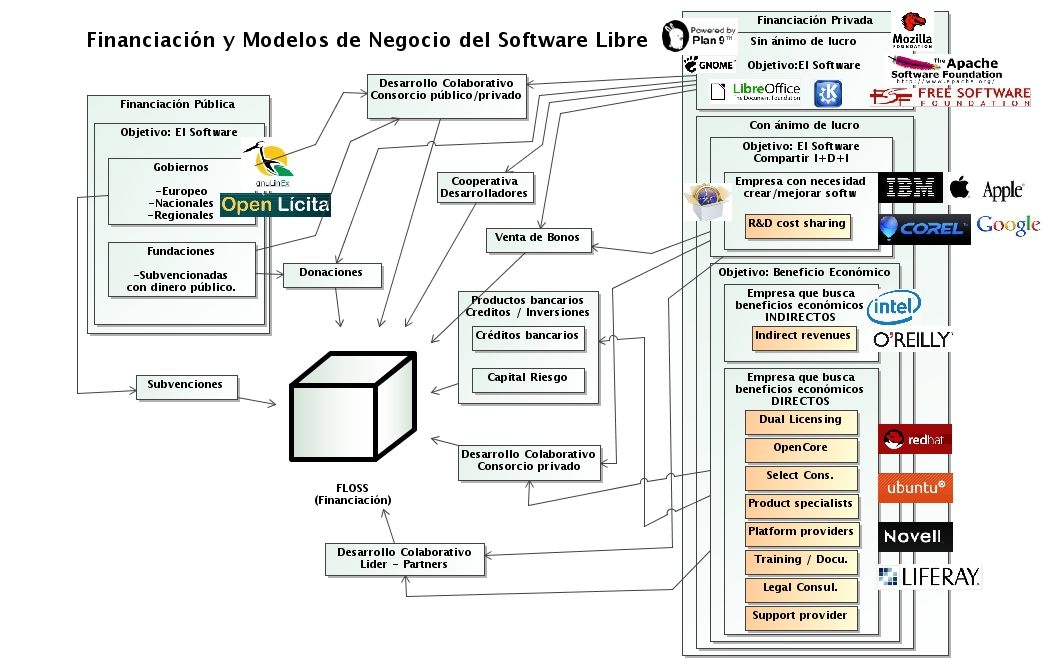
\includegraphics[width=\textwidth]{./MSWL-CSII-ModelosNegocioFlossDHernandez-ACarmona.jpg}
\end{figure}
   
\end{document}
